\documentclass{spanish_summary}

\begin{document}

\chapter*{Zeit}
\section*{Allgemein}
\begin{longtable}{p{.20\textwidth} | p{.50\textwidth}} 
\textbf{Zeit}     & \textbf{el tiempo}                                       \\ \hline
\hline
\endhead % all the lines above this will be repeated on every page
Sekunde & el segundo\\
Minute & el minuto\\
Stunde & la hora\\
Tag & el dia\\
Woche & la semana\\
Wochenende & el fin de semana\\
Monat & el mes\\
Jahr & el a\~{n}o\\
Jahrhundert & el siglo \\

\end{longtable}

\section*{Monatsnamen}
\begin{longtable}{p{.20\textwidth} | p{.50\textwidth}} 
\textbf{Monatsnamen}     & \textbf{los nombres de los meses}                                       \\ \hline
\hline
\endhead % all the lines above this will be repeated on every page
Januar & el enero\\
Februar & el febrero\\
März & el marzo\\
April & el abril\\
Mai & el mayo\\
Juni & el junio\\
Juli & el julio\\
August & el agosto\\
September & el septiembre\\
Oktober & el octubre\\
November & el noviembre \\
Dezember & el diciembre \\
\end{longtable}

\section*{Jahreszeiten}
\begin{longtable}{p{.20\textwidth} | p{.50\textwidth}} 
\textbf{Jahreszeit}     & \textbf{la estación}                                       \\ \hline
\hline
\endhead % all the lines above this will be repeated on every page
Frühling & la primavera \\
Sommer & el verano \\
Herbst & el oto\~{n}o \\
Winter & el invierno \\
\end{longtable}

\newpage

\section*{Wochentage}
\begin{longtable}{p{.20\textwidth} | p{.50\textwidth}} 
\textbf{Wochentage}     & \textbf{los día de la semana}                                       \\ \hline
\hline
\endhead % all the lines above this will be repeated on every page
Montag & el lunes \\
Dienstag & el martes\\
Mittwoch & el miercoles \\
Donnerstag & el jueves \\
Freitag & el viernes\\
Samstag & el sabado \\
Sonntag & el domingo \\
\end{longtable}
Regelmäßig stattfindende Ereignisse werden üblicherweise durch den Plural des Wochentages gebildet, besipielsweise: "jeden Montag - los lunes, jeden Dienstag - los martes usw."

\section*{Zeitadverbien}
\begin{longtable}{p{.20\textwidth} | p{.50\textwidth}} 
\textbf{~}     & \textbf{~}                                       \\ \hline
bald & pronto\\
gestern & ayer\\
gestern Abend & anoche\\
heute & hoy\\
letzte, -s, -n ... & el mes pasado \newline la semana passado\newline el a\~{n}o passado\\
morgen & ma\~{n}ana\\
vorgestern & anteayer
\end{longtable}

\section*{Datumsangaben}
\subsection*{Muster}
\begin{center}
  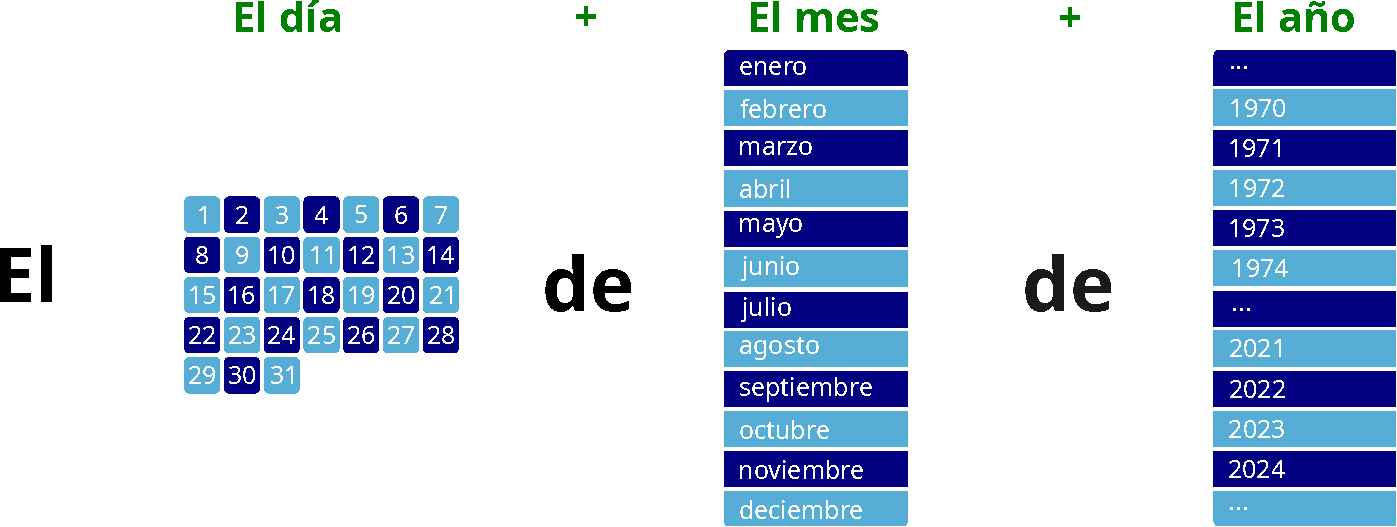
\includegraphics[scale=0.6]{datum.pdf}
\end{center}


\subsection*{Beispiele}
\begin{itemize}
  \item \textbf{1. Januar: } primero de enero
  \item \textbf{15. April 1978: } quince de abril de mil novecientos setenta y ocho
  \item \textbf{3. November 2023: } tres de noviembre de dos mil veintitres
\end{itemize}

\newpage

\section*{Uhrzeit}

\begin{center}
  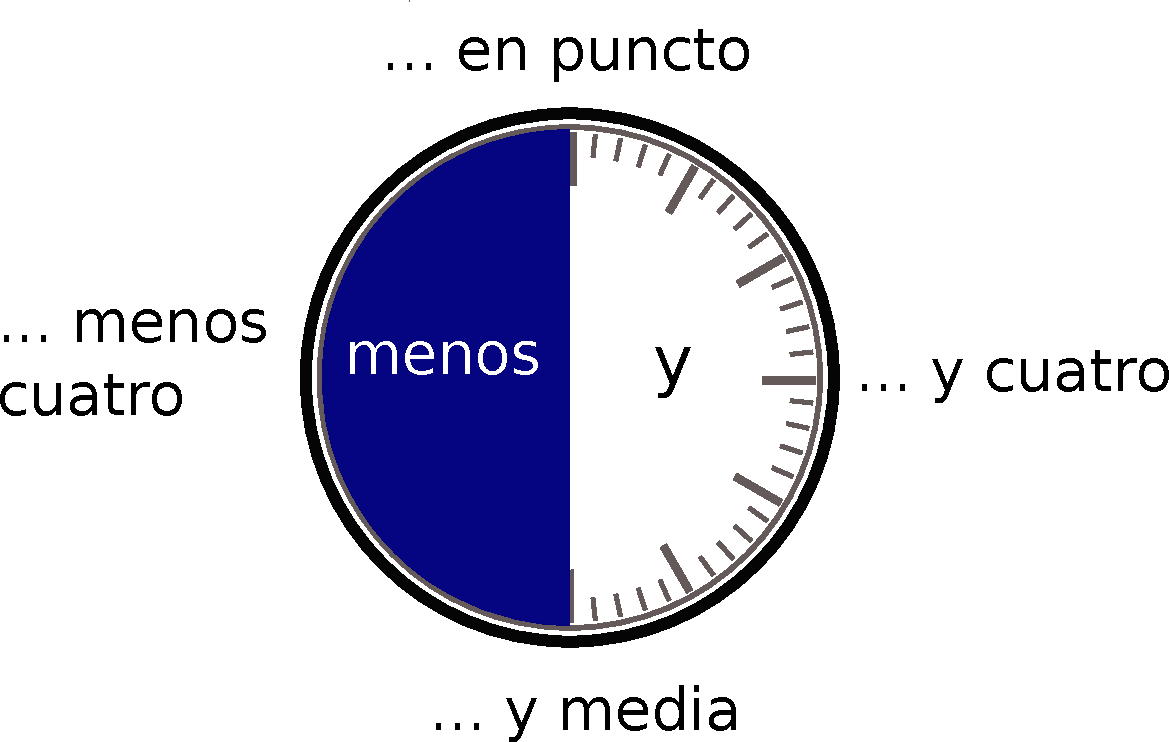
\includegraphics[scale=0.6]{uhrzeit.pdf}
\end{center}

\subsection*{Tagesabschnitte}
\begin{longtable}{p{.20\textwidth} p{.20\textwidth}} 
  frühmorgens & ... por la madrugada \\
  morgens & ... por la ma\~{n}ana \\
  mittags & ... del mediodía \\
  nachmittags & ... por la tarde \\
  abends/nachts & ... por la noche
\end{longtable}

\subsection*{Beispiele}
\begin{itemize}
  \item \textbf{8:05 morgens:} ocho y cinco de la ma\~{n}ana 
  \item \textbf{12:00 mittags:} doce en puncto (del mediodía)
  \item \textbf{2:15 nachmittags:} dos y cuatro de la tarde
  \item \textbf{3:30:} tres y media
  \item \textbf{4:37:} cinco menos veintitres
  \item \textbf{5:45:} seis menos cuatro
\end{itemize}

\renewcommand{\arraystretch}{2} % Nur für diese Tabelle

\section*{Zeiträume}
\begin{tabular}{p{.10\textwidth} | p{.30\textwidth} | p{.32\textwidth}}
~ & \textbf{Verwendung} & \textbf{Beispiel}\\  \hline  \hline
\textbf{hace} & \raggedright Bei einer \underline{einmaligen abgeschlossene} \underline{Handlung} in der Vergangenheit & Llegué hace dos horas a la oficina\\
\textbf{desde} & \raggedright Bei dem \underline{Zeitpunkt} einer Handlung die in der Vergangenheit begonnen hat und immer noch andauert & Vivo en Alemania desde 2010.\newline Trabajo en esta empresa desde 2020\newline Estoy trabajando desde las siete de la mañana. \\
\textbf{desde hace} & Bei einem \underline{Zeitraum} einer Handlung die in der Vergangenheit begonnen hat und immer noch andauert & \raggedright Estudio español desde hace seis meses

\renewcommand{\arraystretch}{1} % Zurück zum Standard

\end{tabular}

\end{document}
